%!TEX root = ../MainBody.tex

% 第一章
\chapter{前言}% 使用\cite{}命令引用数据库中文献
本文档是《川大硕博学位论文~\LaTeX~模板v1.0beta版本》的说明文档。

本LaTeX模板是在Legendary L.\footnote{Legendary Leo \url{https://github.com/cuiao}}于2016年的四川大学学位论文模板\cite{Legendarygit2016}的基础上进行修改的。而LegendaryLeo的四川大学学位论文的工作,以前由~dahakawang\footnote{\url{https://github.com/dahakawang/scu_thesis_template}}~、~tan\footnote{\url{http://www.codeforge.com/article/382397}}~等人做过,是在参考~Casper Ti. Vector\footnote{\url{CasperVector@gmail.com}}~~\emph{pkuthss}~模版\cite{pkuthss}的基础上完成的。在此一并感谢。


Bingo G.\footnote{Bingo Go \url{}}是本文档的创建者和维护者。
\section{模板基础}

\par Legendary基本实现了学位论文的基本功能及格式,开了一个好头。但是在鄙人在对照四川大学研究生院硕博论文毕业要求\cite{si2010si}时,可能由于Legendary模板是基于2009年版的论文要求的原因\cite{SCUDissertationFormat},原模板有诸多不完美的地方,经过针对每个问题就行多番搜索和尝试之后,整理出本版的硕博学位论文模板,因为还是有些许地方不够确定,特将此版本命名为四川大学硕博学位论文LaTeX模板-v1.0beta,同时新建了项目,方便各位同学搜索查看与使用。

\section{适用对象}
经过粗略的对川大硕博学位论文要求与本科学位论文要求进行对比,发现在版面要求上有较多的不同,本模板\textbf{主要对标川大硕博学位论文要求,不推荐本科同学直接使用本模板},本科同学可以使用github上其他项目,或在本项目基础上做出相应修改才能满足要求。

\section{特点与改进}
首先在继承Legendary模板简单方便与自动化程度高的特点的基础上,高度符合《四川大学硕士、博士学位论文格式(2010版)》\cite{si2010si}。对原版本主要进行了一下几个方面的修改:
\begin{itemize}
	\item 页面设置:修改了页面设置及部分页码设置问题。
	\item 页眉页脚:根据模板要求对页眉页脚进行一些调整。
	\item 标题文献等:根据模板要求也做了适当调整。
\end{itemize}

\section{推荐配置}
笔者具体的配置其实忘记了(不要打我),只是遇到一个问题解决一个,大致的需要以下一些要求:
\begin{itemize}
	\item 中文支持:我貌似暗转的CTeX,支持中文。
	\item 编辑器:个人推荐TeXstudio,界面很不错,界面如\cref{fig_jiemian}。
\end{itemize}

具体的安装教程请自行百度。
\begin{figure}[h]
	\centering
	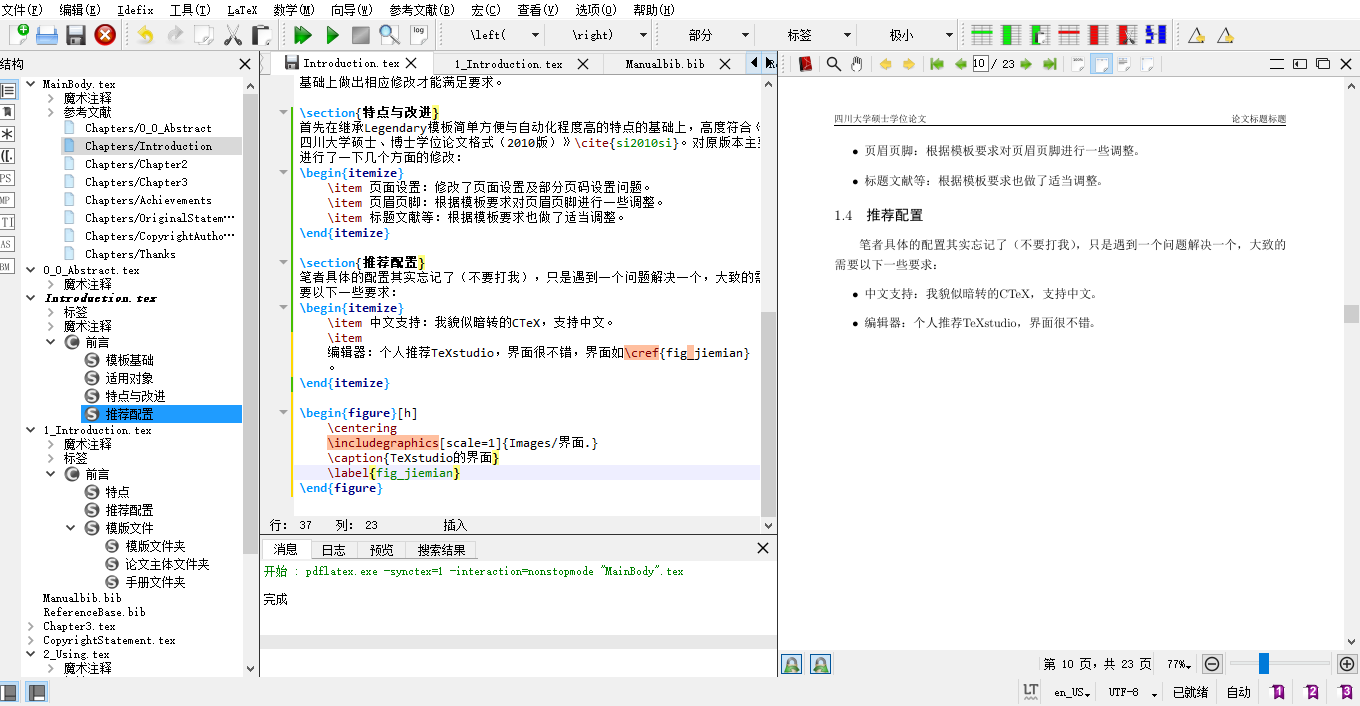
\includegraphics[width=1.0\linewidth]{Images/jiemian.png}
	\caption{TeXstudio的界面}
	\label{fig_jiemian}
\end{figure}
